\documentclass{report}
\usepackage{amsmath}
\usepackage{amssymb}
\usepackage[a4paper, total={7in,10in}]{geometry}
\usepackage{multicol}
\usepackage{graphicx}
\usepackage{enumitem}

\begin{document}
\newcommand{\sol}[1]{
    \noindent \textbf{Sol.}
}
\def\eos{\quad\hbox{\rlap{\hbox{\vrule depth 1.5pt height 2.6mm width 0.2mm \hskip 1mm \vrule height 2.6mm width 0.2mm}}{\vbox{\hrule height 0.2mm width 1.4mm \vskip 2.8mm \hrule depth 1.5pt height -0.35mm width 1.2mm}}}}
\begin{multicols}{2}
    \begin{enumerate}
        \item What is $\dfrac{20 \cdot 22}{(2+0)\cdot(2+2)}$?

              \sol{}
              \begin{flalign*}
                  \dfrac{20 \cdot 22}{(2+0)\cdot(2+2)} & = \dfrac{20 \cdot 22}{2\cdot4}  \\
                                                       & = \dfrac{440}{8}                \\
                                                       & = 55 \ \text{\textbf{(D)}} \eos
              \end{flalign*}

        \item Karo has a box of matches with 30 matches. Using some of the matches she forms
              the number 2022. She has already formed the first two digits (see picture). How
              many matches will be left in the box when she has finished the number?
              \begin{center}
                  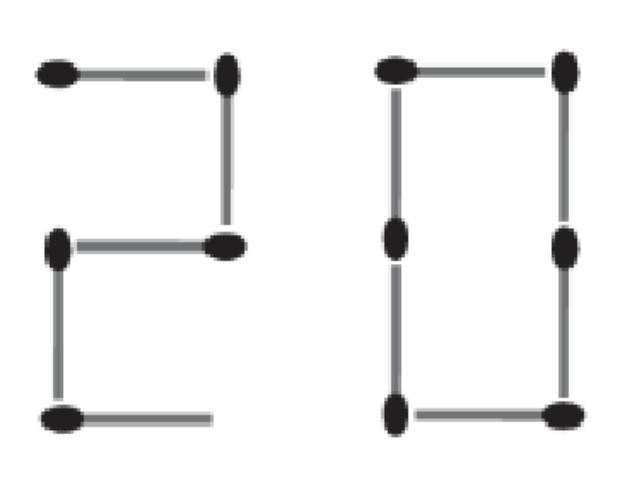
\includegraphics[width=0.2\textwidth]{pictures/1.png}
              \end{center}

              \sol{}

              There are 5 matches in the digit 2 and 6 matches in the digit 0. Therefore, the
              total number of matches required to form the number 2022 is $5 \cdot 3 + 6 =
                  21$.

              Hence, the number of matches left in the box is $30 - 21 = 9$. \textbf{(B)}
              $\eos$

        \item An equilateral triangle with side length 12 has the same perimeter as a square
              with side length $x$. What is the value of $x$?

              \sol{}

              The perimeter of an equilateral triangle is $3 \cdot 12 = 36$. Since the square
              has the same perimeter, the side length $x$ of the square is $\dfrac{36}{4} =
                  9$. \textbf{(A)} $\eos$

        \item Various symbols are drawn on a piece of paper (see picture).

              \begin{center}
                  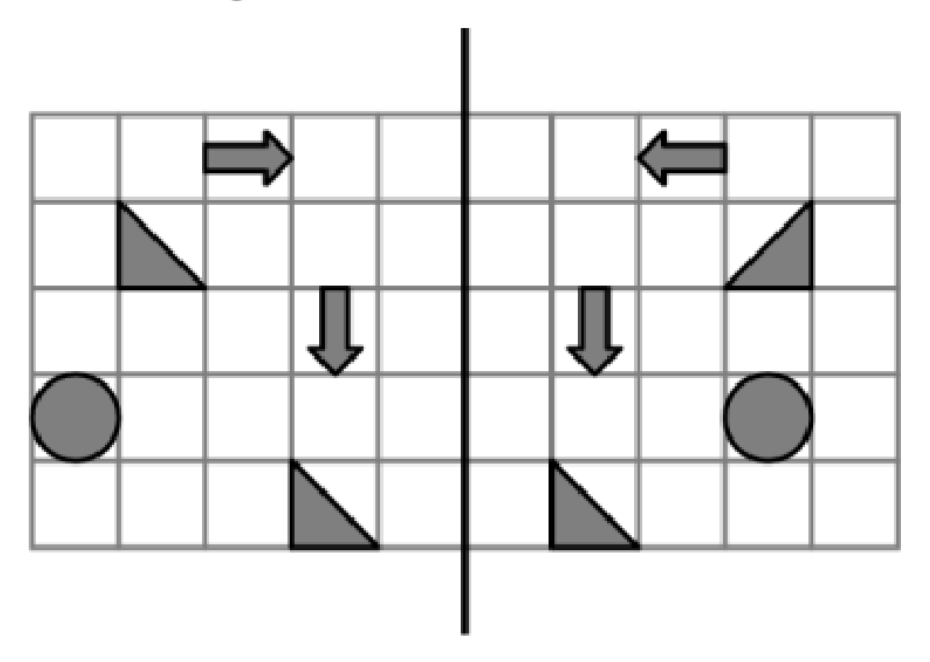
\includegraphics[width=0.3\textwidth]{pictures/2.png}
              \end{center}

              The teacher folds the left side along the vertical line to the right.

              How many symbols of the left side are now congruent on top of a symbol on the
              right side?

              \sol{}

              From top to bottom,

              The arrow on the left and the right side are 3 units away from the symmetry
              line, and they are flipped horizontally. Therefore, they are congruent when the
              the paper is fold.

              The triangle on the left and the right side are 4 units away from the symmetry
              line, and they are flipped horizontally. Therefore, they are congruent when the
              paper is fold.

              The arrow on the left and the right side are 2 units away from the symmetry
              line, and they are the same when being flipped horizontally. Therefore, they
              are congruent when the paper is fold.

              The circle on the left side is 5 units away from the symmetry line, while the
              circle on the right side is 4 units away from the symmetry line. Therefore,
              they are not congruent when the paper is fold.

              The triangle on the left side and the right side are 2 units away from the
              symmetry line, but they are of the same rotation. Therefore, they are not
              congruent when the paper is fold.

              Hence, there are 3 congruent symbols when the paper is fold. \textbf{(C)}
              $\eos$

        \item Karin places a table of size $2 \times 1$ according to the number of
              participants in a meeting. The diagram shows the table arrangements from above
              for a small, medium and a large meeting.

              How many tables are used in a large meeting?

              \begin{center}
                  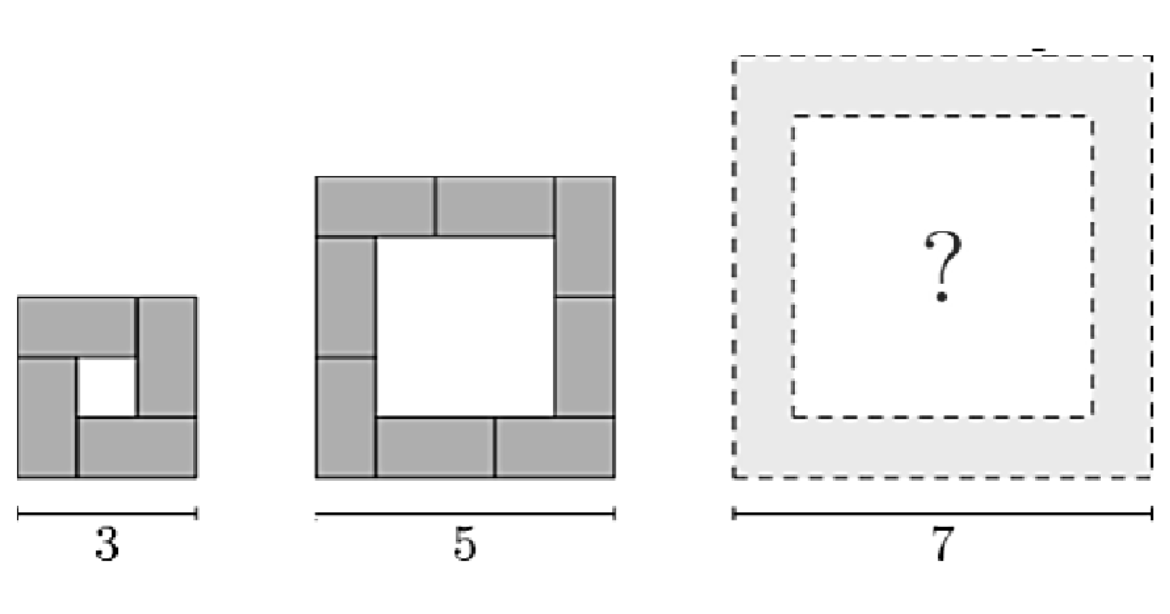
\includegraphics[width=0.36\textwidth]{pictures/3.png}
              \end{center}

              \sol{}

              In each arrangement, the table required is $\dfrac{n-1}{2} \cdot 4$, where $n$
              is the side length of the arrangement. Therefore, the number of tables required
              in the large meeting is $\dfrac{7-1}{2} \cdot 4 = 12$. \textbf{(C)} $\eos$

        \item I am smaller than my half and bigger than my double. The sum of me and my
              square is 0.

              \sol{}

              Let $x$ be the number. Then, we have the following statements:
              \begin{flalign*}
                  \text{I am smaller than my half}        & \implies x < \dfrac{x}{2} \\
                  \text{I am bigger than my double}       & \implies x > 2x           \\
                  \text{The sum of me and my square is 0} & \implies x + x^2 = 0
              \end{flalign*}
              \begin{flalign*}
                  \because 2x < x < \dfrac{x}{2} \implies x < 0 \\
                  \because x + x^2 = 0 \implies x = -1 \text{ \textbf{(B)}} \eos
              \end{flalign*}

        \item The midpoints of both longer sides of a rectangle are connected with the
              vertices (see diagram).
              \begin{center}
                  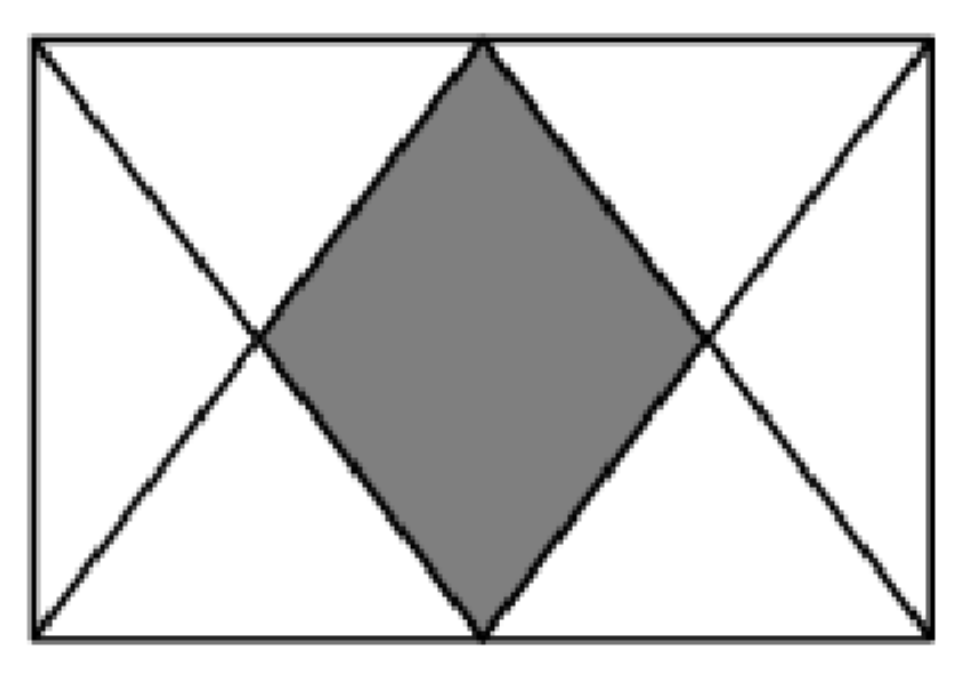
\includegraphics[width=0.28\textwidth]{pictures/4.png}
              \end{center}
              Which fraction of the rectangle is shaded?

              \sol{}

              Splitting the rectangle into eight equal parts, each part is split into two
              equal triangles, as shown below.
              \begin{center}
                  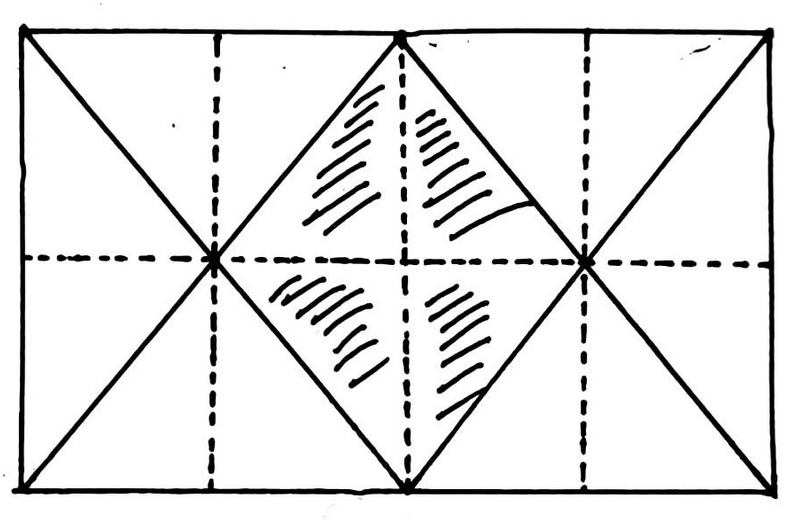
\includegraphics[width=0.28\textwidth]{pictures/5.png}
              \end{center}
              There are 16 triangles in total, while the shaded area consists of 4 triangles. Hence, the fraction of the rectangle that is shaded is $\dfrac{4}{16} = \dfrac{1}{4}$. \textbf{(B)} $\eos$

        \item Sonja's smartphone displays the diagram on the right. It shows how long he has
              worked for four different apps in the previous week. This week he has spent
              only half the amount of time using two of the apps and the same amount of time
              as last weeks using the other two apps. Which of the following pictures could
              be the diagram for the current week?
              \begin{center}
                  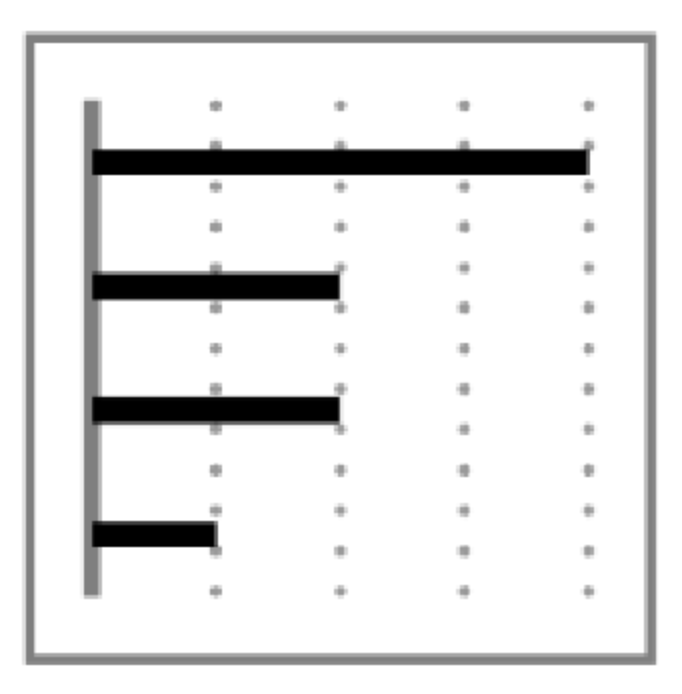
\includegraphics[width=0.24\textwidth]{pictures/6.png}
              \end{center}

              \sol{}

              From the picture, from top to bottom, the time spent on the apps are 4, 2, 2, 1
              respectively. In the options:
              \begin{enumerate}[label=(\Alph*)]
                  \item 2 (half), 1(half), 1(half), 0.5 (half)
                  \item 4, 2, 1 (half), 1
                  \item 2 (half), 2, 1 (half), 1
                  \item 3 (three quarter), 1 (half), 1 (half), 0.5 (half)
                  \item 2 (half), 1 (half), 1 (half), 1
              \end{enumerate}
              Hence, the correct answer is \textbf{(C)}. $\eos$

        \item In the multiplication grid displayed, each white cell should show the product
              of the numbers on the grey cells that are in the same row and column
              respectively. One number is already entered. The integer $x$ is bigger than the
              positive integer $y$. What is the value of $y$?

              \sol{}

              \begin{center}
                  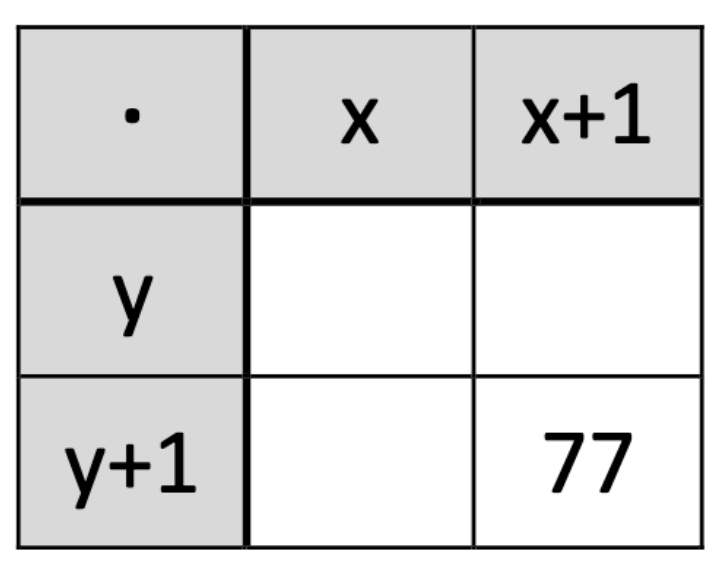
\includegraphics[width=0.24\textwidth]{pictures/7.png}
              \end{center}

              If $y = 6$, $y + 1 = 7$, $x + 1 = 77 \div 7 = 11$, $x = 10$.

              If $y = 7$, $y + 1 = 8$, $x + 1 = 77 \div 8 = 9.625$, $x = 8.625$.

              If $y = 8$, $y + 1 = 9$, $x + 1 = 77 \div 9 = 8.555$, $x = 7.555$.

              If $y = 10$, $y + 1 = 11$, $x + 1 = 77 \div 11 = 7$, $x = 6$.

              If $y = 11$, $y + 1 = 12$, $x + 1 = 77 \div 12 = 6.416$, $x = 5.416$.

              Since $x, y \in \mathbb{Z^+}$, $x > y$, $y = 6$ is the only possible answer.
              \textbf{(A)} $\eos$

        \item There are 5 people to choose from on a ballot paper. After counting 90\% of the
              votes in the intermediate results looks as shown in the table. How many of the
              5 people cannot win the election anymore?
              \begin{center}
                  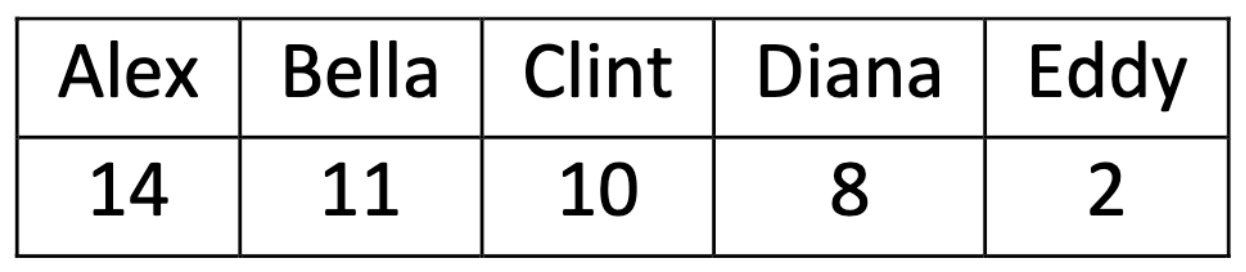
\includegraphics[width=0.33\textwidth]{pictures/8.png}
              \end{center}

              The number of votes counted is $14 + 11 + 10 + 8 +2 = 45$. The number of votes
              haven't been counted yet is $45 \div \dfrac{100}{90} \cdot \dfrac{10}{100} =
                  5$.

              After all the votes are counted, if all the previously uncounted votes are for
              the same person, then

              For Alex, he will get $14 + 5 = 19$ votes, which is enough to win the election.

              For Bella, she will get $11 + 5 = 16$ votes, which is enough to win the
              election.

              For Clint, he will get $10 + 5 = 15$ votes, which is enough to win the
              election.

              For Diana, she will get $8 + 5 = 13$ votes, which is not enough to win the
              election.

              For Eddy, he will get $2 + 5 = 7$ votes, which is not enough to win the
              election.

              Hence, the number of people who cannot win the election is $2$. \textbf{(B)}
              $\eos$

        \item Five squares and two right-angled triangles are placed as shown in the diagram.
              The number 3, 8, 22 in the squares state the size of the area in
              \textit{m}$^2$. How big is the area (in \textit{m}$^2$) of the square with the
              question mark?

              \sol{}

              \begin{center}
                  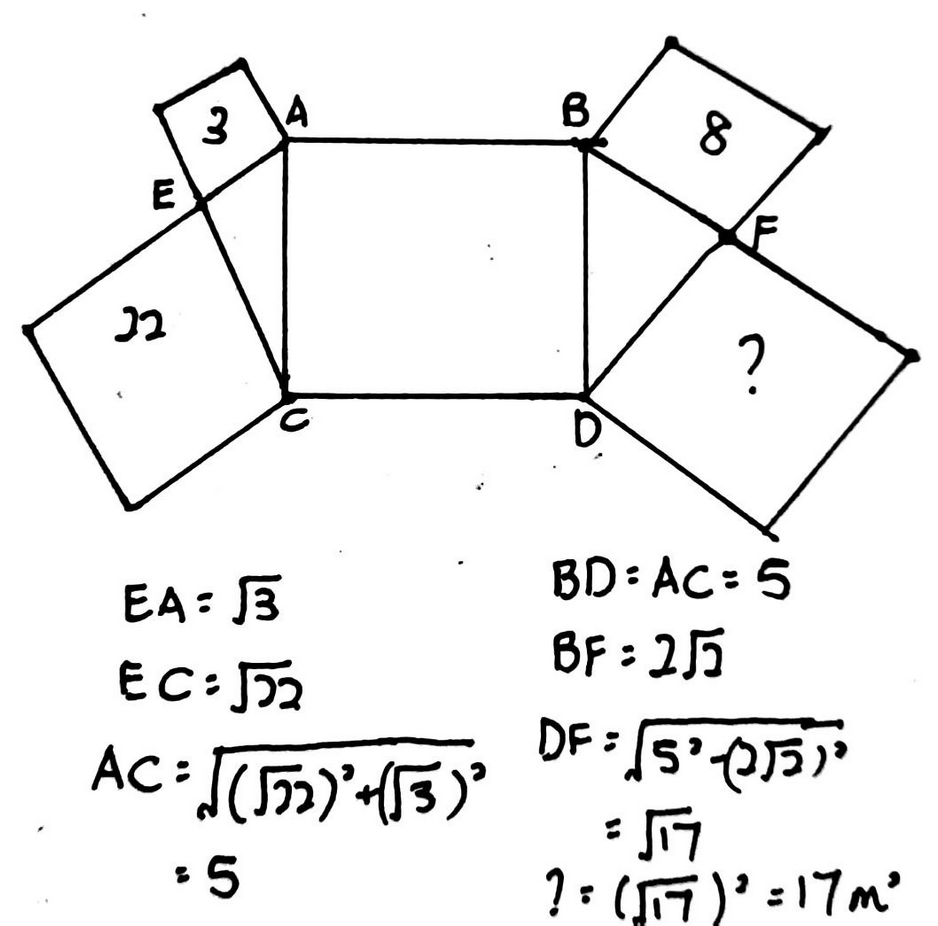
\includegraphics[width=0.36\textwidth]{pictures/9.png}
              \end{center}

              The area of the square with the question mark is $17\textit{m}^2$. \textbf{(D)}
              $\eos$

        \item 2022 tiles are placed in one long row. Adam removes every sixth tile. Then Beate removes every fifth of the remaining tiles.

              Subsequently Cora removes every fourth of the remaining tiles.

              How many tiles are left?

              \sol{}

              For Adam, he removes $2022 \div 6 = 337$ tiles.

              For Beate, she removes $(2022 - 337) \div 5 = 337$ tiles.

              For Cora, she removes $(2022 - 337 - 337) \div 4 = 337$ tiles.

              Hence, the number of tiles left is $2022 - 3 \times 337= 1011$. \textbf{(A)}
              $\eos$

        \item The diagram shows three big circles of equal size and four small circles. Each
              small circle touches two big circles and has radius 1.

              How big is the shaded area?
              \begin{center}
                  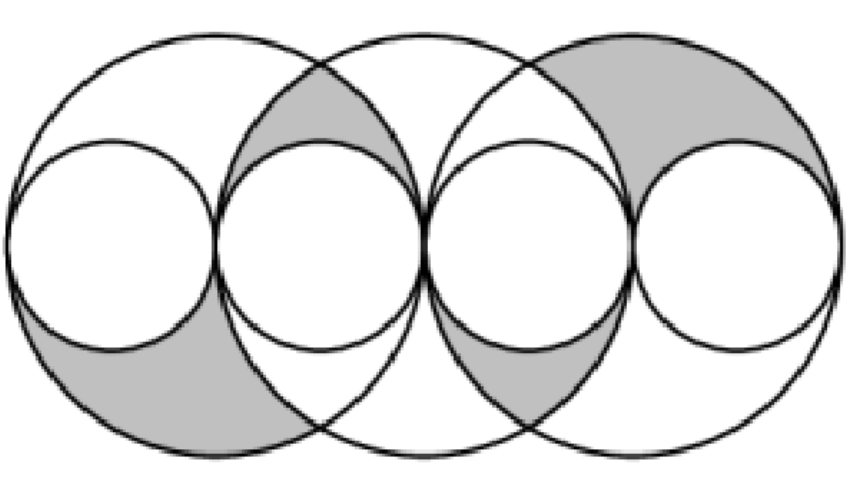
\includegraphics[width=0.3\textwidth]{pictures/10.png}
              \end{center}

              \sol{}

              Move the bottom two shaded area to the top, and draw a line separating shape
              into top and bottom parts, we get the following:
              \begin{center}
                  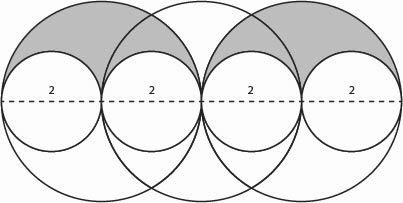
\includegraphics[width=0.33\textwidth]{pictures/12.jpg}
              \end{center}
              Having inspected the diagram, we can see that there are two shaded region, the area of each of them is the area of a big semicircle minus 2 times the area of a small semicircle:
              \begin{flalign*}
                  \text{Area of the small semicircle} & = \dfrac{1}{2} \pi \times 1^2 = \dfrac{\pi}{2} \\
                  \text{Area of the big semicircle}   & = \dfrac{1}{2} \pi \times 2^2 = 2\pi           \\
                  \text{Area of the shaded region}    & = 2\pi - 2 \times \dfrac{\pi}{2} = \pi
              \end{flalign*}
              Since there are two shaded region, the total area of the shaded region is $2 \times \pi = 2\pi$. \textbf{(B)} $\eos$

        \item A bee called Maja wants to hike from honeycomb $X$ to honeycomb $Y$. Sje can
              only move from one honeycomb to the neighbouring honeycomb if they share an
              edge. How many, different ways are there for Maja to go from $X$ to $Y$ if she
              has to step onto every one of the seven honeycombs exactly once? \sol{}

              \begin{center}
                  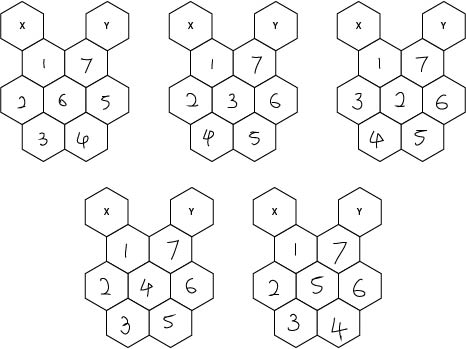
\includegraphics[width=0.36\textwidth]{pictures/13.jpg}
              \end{center}
              After some manual calculation, there are 5 different ways for Maja to achieve her goal. \textbf{(D)} $\eos$

        \item The sum of two positive integers is three times as big as their difference.

              The product of the two numbers is four times as big as their sum.

              How big is the sum of the two numbers?

              \sol{}

              Let the two numbers be $x$ and $y$, $x > y > 0$.
              \begin{flalign*}
                  x+y & = 3(x-y) \quad \cdots\ (1) \\
                  xy  & = 4(x+y) \quad \cdots\ (2)
              \end{flalign*}
              \begin{flalign*}
                  (1)\ \Rightarrow \ x+y & = 3x - 3y \\
                  2x - 4y                & = 0       \\
                  x                      & = 2y
              \end{flalign*}
              \begin{flalign*}
                  (2)\ \Rightarrow \ xy & = 4x + 4y \quad \cdots\ (4) \\
              \end{flalign*}
              Substituting $x = 2y$ into $(4)$, we get
              \begin{flalign*}
                  (2y)(y)  & = 4(2y) + 4y                     \\
                  2y^2     & = 8y + 4y                        \\
                  2y^2     & = 12y                            \\
                  y^2 - 6y & = 0                              \\
                  y(y-6)   & = 0                              \\
                  y        & = 6\ (y > 0)                     \\
                  x        & = 2 \times 6 = 12                \\
                  x + y    & = 12 + 6 = 18\ \textbf{(E)} \eos
              \end{flalign*}

        \item The rectangle $ABCD$ is made up of 12 congruent rectangles (see diagram).

              How big is the ratio $\dfrac{AD}{DC}$?
              \begin{center}
                  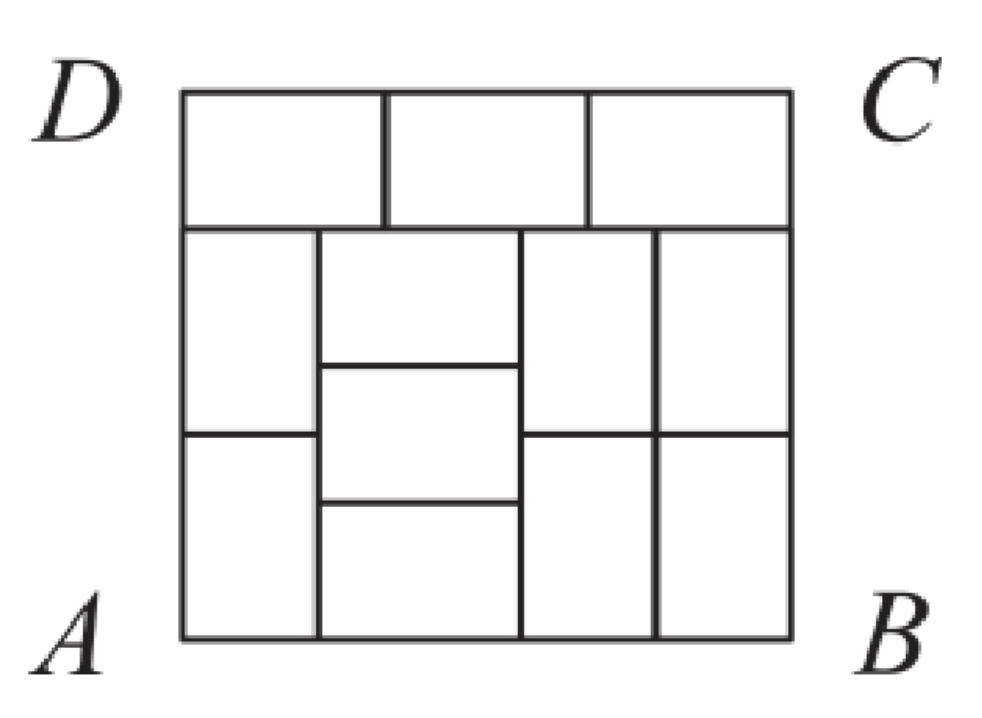
\includegraphics[width=0.28\textwidth]{pictures/14.png}
              \end{center}

              \sol{}

              Each rectangle can be divided into three parts horizontally and two parts
              vertically:
              \begin{center}
                  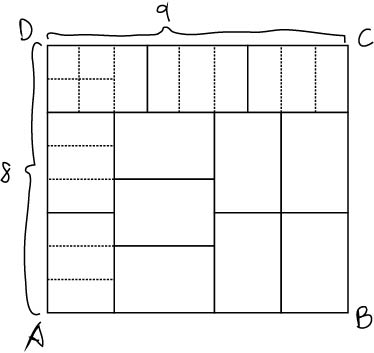
\includegraphics[width=0.3\textwidth]{pictures/15.jpg}
              \end{center}

              Therefore, the ratio $\dfrac{AD}{DC}$ is $\dfrac{8}{9}$. \textbf{(A)}

        \item A rabbit and a hedgehog enter a race against each other. The circular
              racecourse is 550\textit{m} long. The starting line and the finish line are the
              same. The speed of the rabbit is a constant 10\textit{m}/\textit{s}, the speed
              of the hedgehog is a constant 1\textit{m}/\textit{s}. They start at the same
              time, but the hedgehog tries to cheat by going in the opposite direction. When
              the two meets, the hedgehog turns around immediately and follows the rabbit.

              How many seconds after the rabbit does the hedgehog reach the finish line?

              \sol{} Let the distance travelled by the hedgehog before meeting the rabbit be $x$.
              \begin{flalign*}
                  x + 10x & = 550           \\
                  11x     & = 550           \\
                  x       & = 50 \textit{m}
              \end{flalign*}
              After the hedgehog turns around, it needs to travel $\dfrac{50\textit{m}}{1\textit{m}/\textit{s}} = 50\textit{s}$ more to reach the finish line, while the rabbit only needs to travel $\dfrac{50\textit{m}}{10\textit{m}/\textit{s}} = 5\textit{s}$ more. Hence, the hedgehog reaches the finish line $50 - 5 = 45\textit{s}$ seconds after the rabbit. \textbf{(A)} \eos

        \item The grandchildren ask their grandma how old she is. The grandma invites them to
              guess the age.

              The first child says 75, the second says 78 and the third says 81. It turns out
              that one child is wrong by 1 year, one by 2 years and one by 4 years. How many
              possibilities are there for the age of the grandma? are there for the age of
              the grandma?

              \sol{}

              If the first child says wrong by 2 years, the actual age of the grandma is 77.
              Which means, the second child is wrong by 1 year, while the third child is
              wrong by 4 years, which is valid.

              If the first child says wrong by 4 years, the actual age of the grandma is 79.
              Which means, the second child is wrong by 4 years, while the third child is
              wrong by 2 years, which is valid.

              The other possibilities are not valid. Hence, there are 2 possibilities for the
              actual age of grandma. \textbf{(C)} $\eos$

        \item There are three paths running through our park in the city (see diagram).
              \begin{center}
                  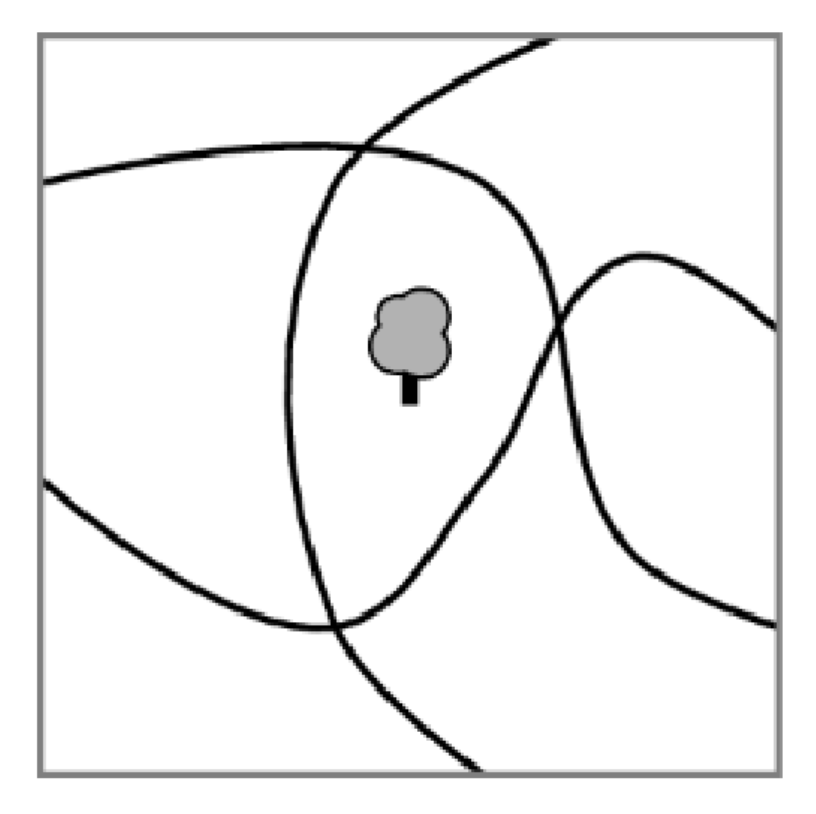
\includegraphics[width=0.3\textwidth]{pictures/16.png}
              \end{center}
              What is the minimum number of trees that have to be planted additionally so that there are the same number of trees on either side of each path?

              \sol{}

              \begin{center}
                  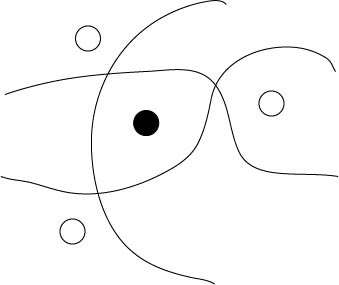
\includegraphics[width=0.3\textwidth]{pictures/17.jpg}
              \end{center}

              With some manual calculation, we can see that the minimum number of trees that
              have to be planted is 3. \textbf{(C)} $\eos$

        \item The diagram shows a square $PQRS$ with side length 1. The point $U$ is the
              midpoint of the side $RS$ and the point $W$ is the midpoint of the square.

              \begin{center}
                  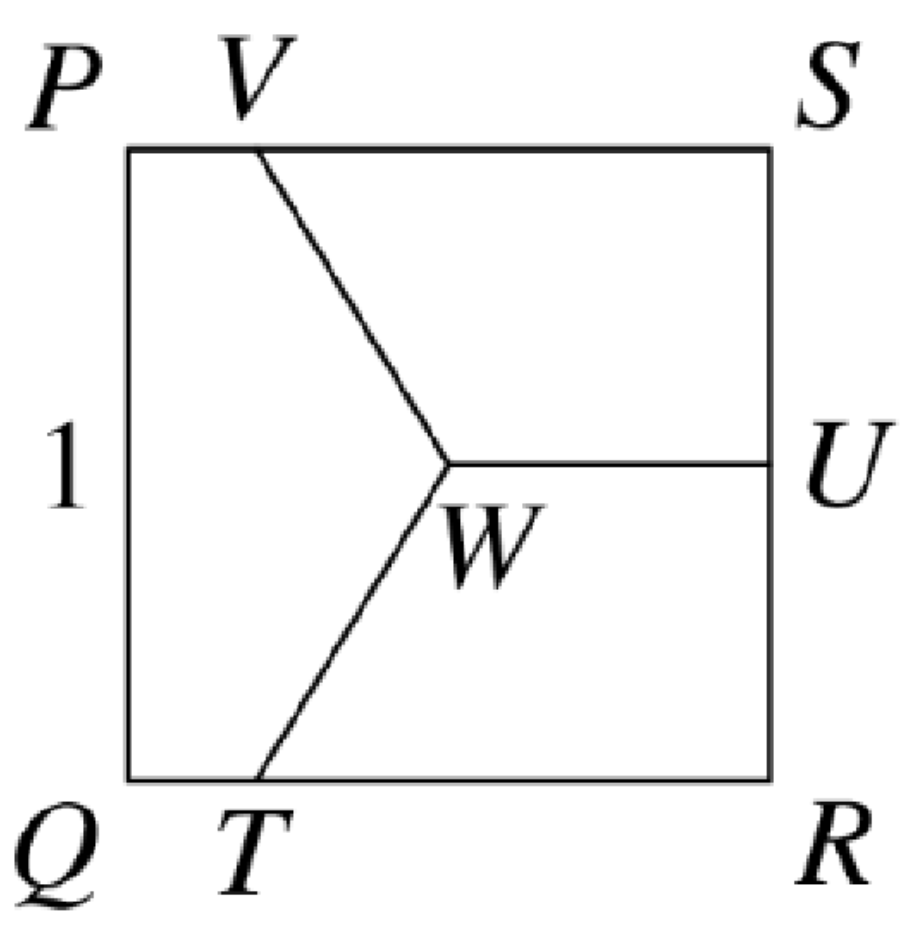
\includegraphics[width=0.25\textwidth]{pictures/18.png}
              \end{center}

              The three line segments, $TW$, $UW$, and $VW$ split the square into three equal
              big areas.

              How long is the line segment $SV$?

              \sol{}

              \begin{center}
                  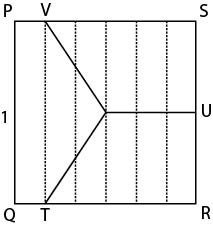
\includegraphics[width=0.23\textwidth]{pictures/19.jpg}
              \end{center}

              The square can be divided horizontally into 6 equal parts. Those, the length of
              the line segment $SV$ is $\dfrac{5}{6}$. \textbf{(E)} $\eos$
    \end{enumerate}
\end{multicols}
\end{document}